\chapter{Fundamentos teóricos} \label{ich:fundamentos_teoricos}

En esta sección introduciremos algunos \textbf{conceptos teóricos} sobre los que se basará nuestro trabajo, y por tanto, conviene conocer para entender este trabajo.

\section{\textit{Embeddings}} \label{isec:embeddings}

Nuestro trabajo busca desarrollar un modelo de aprendizaje automático que aprenda un \textit{embedding}. Un \textit{embedding} no es más que un mapeo desde un cierto espacio $X$ de datos de entrada (en nuestro caso, podemos considerar $X$ como el espacio de imágenes en las que aparecen caras) a un espacio vectorial $\R^N$. En la mayoría de casos, la dimensión del espacio de llegada $N$ es menor que la dimensión del espacio $X$.

Más formalmente, buscamos aprender una función

\begin{equation}
\begin{split}
    f_{\theta}: X & \to \R^N \\
    x & \mapsto f_{\theta}(x)
\end{split}
\end{equation}

que tomamos de una familia paramétrica de funciones $\{f_{\theta}: \theta \in \Theta \}$. En el caso de nuestro problema, podemos pensar en la familia de los modelos profundos de redes convolucionales ($\theta$ estaría por tanto compuesto por todos los coeficientes que determinan dicho modelo convolucional, luego podríamos pensar en $\Theta \subseteq \R^M$ donde $M$ es el número de coeficientes del modelo).

El criterio para escoger una función u otra de mapeo es que este deberá ser \textbf{semántico}. En el espacio de llegada $\R^N$ tenemos una métrica:

\begin{equation}
\begin{split}
    D: X \times X & \to [0, \infty) \\
    x, y & \mapsto D(x, y)
\end{split}
\end{equation}

Por ejemplo, la métrica euclídea. Queremos que \textbf{datos semánticamente relacionados en $X$ sean mapeados a vectores en $\R^N$ cercanos} por la métrica que fijemos. Del mismo modo, datos semánticamente distintos deberán ser mapeados a vectores distantes.

Además, será deseable que $f_{\theta}$ sea una función continua (en casi cualquier ámbito podemos considerar $X = \R^M$ para algún valor de $M$). Por ejemplo, en el caso de las imágenes, un ligero cambio en un \textit{píxel} de la imagen no debería producir un vector muy distanciado del original. En muchas ocasiones, al estar buscando que el \textit{embedding} sea semántico, esta restricción inducirá en menor o mayor medida dicha continuidad.

\begin{ejemplo}
    Consideremos que queremos computar un \textit{embedding} para representar palabras.

    Este problema es \textbf{especialmente relevante} en el ámbito del lenguaje natural. Esto es así porque, si queremos trabajar con texto usando modelos de aprendizaje automático, deberemos primero convertir dicho texto a una representación numérica. Usar, por ejemplo, el código binario que codifica dicho texto no parece muy buena idea, porque este mapeo no es semántico ni continuo.

    En este caso, queremos que palabras con una semántica parecida se transformen a vectores cercanos. Por ejemplo, la distancia entre los \textit{embeddings} de las palabras \entrecomillado{ciudad}, \entrecomillado{pueblo} debería ser mucho menor que la distancia entre los \textit{embeddings} de las palabras \entrecomillado{papel}, \entrecomillado{odio}. Esta idea se puede visualizar en la siguiente representación:

    \begin{figure}[H]
        \centering
        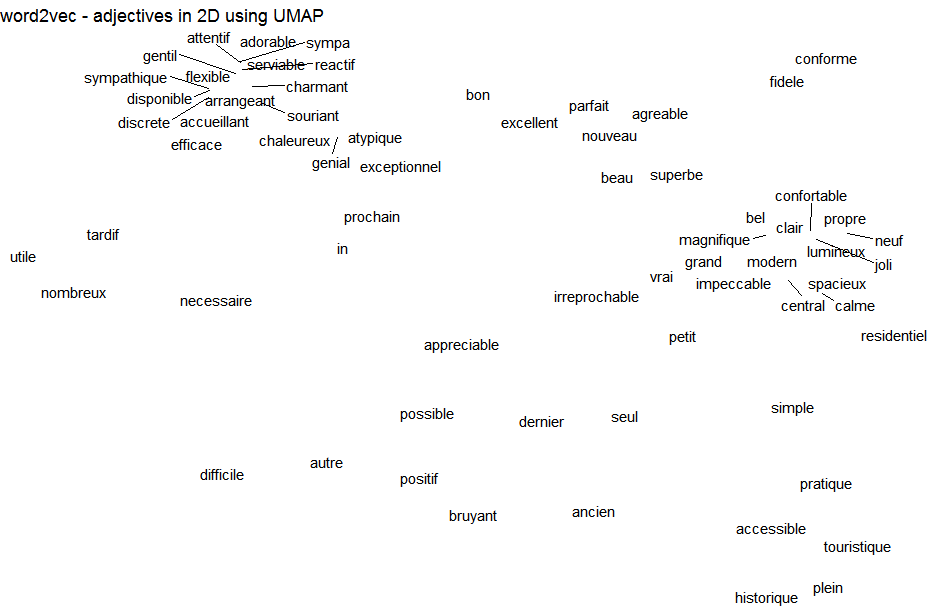
\includegraphics[width=0.6\textwidth]{informatica/word2vec_example}
        \caption{Ejemplo de un \textit{embedding} semántico, computado por el modelo \textit{word2vec} \cite{informatica:word2vec}, de palabras en francés. Imagen extraída de \url{https://cran.r-project.org/web/packages/word2vec/readme/README.html}}
    \end{figure}

    En el caso concreto de \cite{informatica:word2vec}, que propone el conocido modelo \textit{word2vec}, se consigue que el \textit{embedding} tenga cierta \entrecomillado{estructura algebraica}, pudiendo computar, por ejemplo:

    \begin{equation}
        vector("rey") - vector("hombre") + vector("mujer") = vector("reiina")
    \end{equation}
\end{ejemplo}

\begin{ejemplo}
    Veamos ahora un ejemplo mucho más cercano con el problema que queremos resolver. Por ejemplo, el problema de re-identificación (ambiente en el que se proponen las nuevas técnicas de cómputo del \textit{triplet loss} \cite{informatica:principal}).

    En este caso, queremos que las imágenes de una persona en una escena, se transformen a vectores cercanos, como muestra la siguiente representación:

    \begin{figure}[H]
        \centering
        \includegraphics[width=0.6\textwidth]{informatica/embedding_paper_principal}
        \caption{Imagen extraída de \cite{informatica:principal}. Se representa una proporción del \textit{dataset} \textit{Market-1501} tras aplicar el \textit{embedding} aprendido y posteriormente \textit{t-SNE}}
    \end{figure}

    Por ejemplo, un modelo que quiera resolver esta tarea podría aprender a mapear personas con exactamente la misma ropa a puntos cercanos.
\end{ejemplo}

\begin{ejemplo}

    Y para finalizar, consideremos nuestra tarea en concreto. Buscamos que las imágenes de la misma persona, aunque hayan pasado los años, se transformen en vectores cercanos. Y al contrario, que imágenes de dos personas distintas estén lo más lejos posible.

    Esto es especialmente complicado, como ya hemos comentando en \customref{ich:descrp_problema}, porque por ejemplo, nuestro modelo debe ver como más cercanos imágenes de un niño y un adulto con barba (ambos siendo la misma persona) que dos imágenes de dos adultos con barba (siendo distintas personas), como hemos mostrado claramente en \customref{img:messi_distintos_otro_adulto}

\end{ejemplo}

\section{\textit{Triplet Loss}} \label{isec:triplet_loss}

Nuestro objetivo es ahora justificar el uso de \textit{triplet loss} como una función de pérdida que permita a nuestro modelo aprender un \textit{embedding} semántico.

Recordemos que estamos trabajando con funciones de la forma:

\begin{equation}
\begin{split}
    f_{\theta}: X & \to \R^N \\
    x & \mapsto f_{\theta}(x)
\end{split}
\end{equation}

y con una métrica:

\begin{equation}
\begin{split}
    D: X \times X & \to [0, \infty) \\
    x, y & \mapsto D(x, y)
\end{split}
\end{equation}

Para ser más concisos, usaremos la notación $D_{i, j} := D(f_{\theta}(x_i), f_{\theta}(x_j))$.

Como su nombre indica, \textit{triplet loss} trabajará sobre triples. Esto es, trabajaremos con:

\begin{enumerate}
    \item Una imagen de un individuo concreto, a la que llamaremos \textbf{\textit{anchor}} o ancla
    \item Otra imagen distinta, pero del mismo individuo, a la que llamaremos \textbf{positivo}
    \item Una imagen de un individuo distinto, a la que llamaremos \textbf{negativo}
\end{enumerate}

En este caso, queremos que la distancia entre el \textit{embedding} del ancla y el positivo (que podemos denotar $D_{A, P}$) sea mucho menor que la distancia entre el \textit{embedding} del ancla y el negativo (denotamos $D_{A, N}$). Por tanto, lo que realmente queremos es que:

\begin{equation}
    D_{A, P} \leq D_{A, N}
\end{equation}

o lo que es lo mismo,

\begin{equation}
    D_{A, P} - D_{A, N} \leq 0
\end{equation}

Una forma trivial de hacer que esa ecuación se cumpla, es haciendo que

\begin{equation}
    f(x) = \vec{0}; \dspace \forall x \in X
\end{equation}

con lo que obtendríamos un modelo totalmente inservible. Para evitar eso, introducimos un término $\alpha > 0$ que se conoce como \textbf{margen}, llegando a:

\begin{equation}
    D_{A, P} - D_{A, N} + \alpha \leq 0
\end{equation}

Buscamos que el término de la izquierda sea lo más negativo posible, por lo buscamos minimizar la siguiente función de pérdida:

\begin{equation}
\begin{split}
    \mathcal{L}_{tri}(A, P, N) & := max \{D_{A, P} - D_{A, N} + \alpha, 0 \} = \ldots \\
    \ldots &= ReLU(D_{A, P} - D_{A, N} + \alpha)
\end{split}
\end{equation}

Minimizando esta función de pérdida, lo que haremos será atraer elementos de la misma clase entre sí, y alejar elementos de clases distintas. Este proceso se refleja en la siguiente imagen:

\begin{figure}[H]
    \centering
    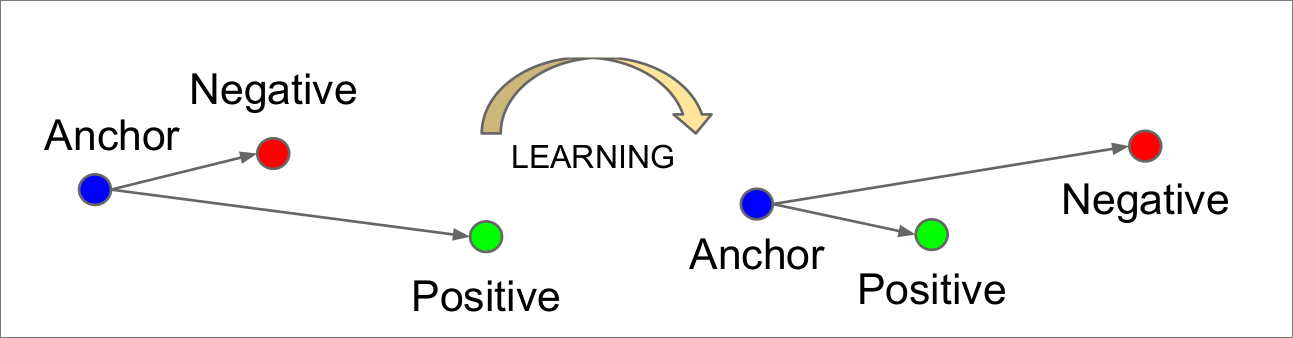
\includegraphics[width=0.8\textwidth]{informatica/triplet_loss_learning}
    \caption{Ejemplo gráfico del proceso de aprendizaje deseado con \textit{triplet loss}. Imagen extraída de \cite{informatica:facenet}}
\end{figure}

\subsection{Ventajas}

A diferencia de otros enfoques basados en usar funciones de pérdida auxiliares (y que fuerzan que la red solo pueda funcionar comparando pares de imágenes), el cómputo del \textit{embedding} es directo una vez entrenado el modelo, siendo muy fácil de adaptar a tareas de \textit{clustering}, \textit{retrieval}, verificación, \ldots \cite{informatica:principal}

Estamos usando un modelo convolucional junto con nuestra función de pérdida para computar directamente el \textit{embedding} deseado, sin funciones de pérdida intermedias que en tiempo de evaluación nunca vamos a usar (\textit{end-to-end learning}) \cite{informatica:principal}

\cite{informatica:principal} comenta que triplet loss es bastante poco popular


\subsection{\textit{Triplet Loss} clásico}



